\documentclass[crop=false]{standalone}
\begin{document}
	\section{Methodology}
	\subsection{System Overview}
	As shown in Figure 1, the system architecture includes a camera mounted on the drone, such as an RGB-D or RGB camera, which captures images. These images are then fed to a deep learning model responsible for object detection. The positions of the detected objects are converted into coordinates and provided to the Dynamic Window Approach (DWA) algorithm for dynamic path adjustment. The output is the optimal path as evaluated by the DWA algorithm. Additionally, shortest path algorithms like $A^*$ and Dijkstra are incorporated to enhance the speed of path selection by the DWA.
	
	\begin{figure*}[thbp!]
		\centering
		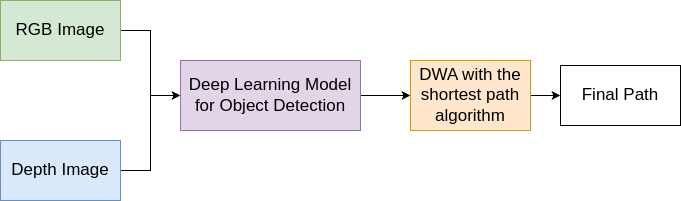
\includegraphics[width=\textwidth]{system_architecture}
		\caption{The system architecture}
		\label{fig:system}
	\end{figure*}
	
	\subsection{General Kinematics Model}
	This study utilizes drones and assumes motion at a fixed altitude and speed, simplifying local path planning problems into 2D path planning problems. DWA transforms the robot's position control problem into a velocity control problem and predicts the robot's motion trajectory through velocity control. To achieve this, the robot's motion model needs to be analyzed \cite{fox}. Let $x(t), y(t)$ denote the robot's pose in the world coordinate system at time $t$, and let $\theta(t)$ represent the direction of the robot. Thus, the robot's motion can be expressed as $<x, y, \theta>$. Let $v$ denote the translational velocity of the robot and $\omega(t)$ denote the angular acceleration. Generally, this can be expressed as follows:
	\begin{equation}
		x(t_n)=x(t_0)+ \int_{t_0}^{t_n}v(t) \cdot cos(\theta)dt
	\end{equation}
	\begin{equation}
		y(t_n)=y(t_0)+ \int_{t_0}^{t_n}v(t) \cdot sin(\theta)dt
	\end{equation}
	\begin{equation}
		\theta(t)=\theta(t_0)+\int_{t_0}^{t_n}\omega(t)dt
	\end{equation}
	\subsection{Objective Function}
	Due to the presence of multiple different translational velocities and angular velocities, it is necessary to select the optimal path from the paths formed by different combinations of translational velocities and angular velocities. The selection process is based on the following objective function:
	\begin{equation}
		G(v, \omega)=\sigma(\alpha Heading(v, \omega) + \beta Obstacle(v, \omega) + \gamma Velocity(v, \omega))
	\end{equation}
	\begin{itemize}
		\item Heading function - This function is used to ensure that the robot advances towards the destination while maintaining its orientation towards it. A smaller value of $\theta$ indicates that the angle between the robot and the destination is smaller.
		\item Obstacle avoidance function - In this study, obstacles are static and generated randomly each time. Given the coordinates of the obstacles, the distance $dist$ between the robot and the obstacle can be calculated using the Euclidean formula. If the distance between the robot and the obstacle is greater than the radius of the robot, it can be considered as no collision occurring.
		\item Velocity function - The translation speed of the robot
	\end{itemize}
	
	The function of $\sigma$ is then normalized across the three functions.
	\begin{equation}
		normalHead(i)=\frac{head(i)}{\sum_{i=1}^{n}{head(i)}}
	\end{equation}
	\begin{equation}
		normalDist(i)=\frac{dist(i)}{\sum_{i=1}^{n}{dist(i)}}
	\end{equation}
	\begin{equation}
		normalVelocity(i)=\frac{velocity(i)}{\sum_{i=1}^{n}{velocity(i)}}
	\end{equation}
	Here, n represents all sampled trajectories, and i denotes the current trajectory being evaluated.
	
	\subsection{Application Scenarios}
	This paper assumes a scenario where drones are flying outdoors, facing static obstacles such as flowers, trees, buildings, etc., as well as dynamic obstacles such as pedestrians, cars, motorcycles, and animals. The algorithm presented in this paper enables route adjustments to avoid these obstacles, paving the way for future applications in drone-based delivery services.
\end{document}